\documentclass{article}
\usepackage[utf8]{inputenc}
\usepackage[danish]{babel}
\usepackage{subfiles}
\usepackage{hyperref}
\usepackage{cite}
\usepackage{graphicx}
\usepackage{float}

\addtolength{\oddsidemargin}{-1cm}
\addtolength{\evensidemargin}{-1cm}
\addtolength{\textwidth}{2cm}
\addtolength{\topmargin}{-1.5cm}
\addtolength{\textheight}{3cm}

\graphicspath{{billeder/}}
\begin{document}
\begin{titlepage}
\begin{center}



\includegraphics[width=0.7\textwidth]{./logo}\\[1cm]

\textsc{\Large Obligatorisk opgave \# 2 i BOSC}\\[0.5cm]

\rule{\linewidth}{0.5mm} \\[0.3cm]
{ \LARGE \bfseries Ooperativsystemer og C\\[0.3cm]}
\rule{\linewidth}{0.5mm} \\[1.5cm]

\begin{minipage}{0.5\textwidth}
\begin{flushleft} \large
\emph{Author:}\\
Tom Mørk Christensen\\
Jonas Elbækgaard Jørgensen
\end{flushleft}
\end{minipage}
\begin{minipage}{0.3\textwidth}
\begin{flushright} \large
\emph{ITU-mail:} \\
\textsc{tmch@itu.dk} \\
\textsc{jelb@itu.dk}
\end{flushright}
\end{minipage}

\vfill

\large 9. oktober 2014

\end{center}
\end{titlepage}
\tableofcontents
\pagebreak

\section{Indledning}
I denne rapport beskrives vor løsning af Obligatorisk Opgave 1 i kurset 'Operativsystemer og C' på IT-Universitet, efteråret 2014. Målet med opgaven er at konstruere en simpel kommandoliniefortolker (eller shell), i stil med f.eks. Unix Bash, og i den sammenhæng demonstrere vores forståelse af systemkald og proceshåndtering, samt lavniveau C programmering. Kommandoliniefortolkeren vil blive omtalt under navnet bosh.\\

I opgaven er stillet en række formelle krav til Bosh’s funktionalitet. For at kunne referere til disse krav i rapporten, er de opsummeret her:\\

\begin{description}
\item[K1:] Bosh skal kunne virke uafhængigt. Du må ikke bruge andre eksisterende shells, f.eks. er det ikke tilladt at anvende et systemkald $system()$ til at starte bash.
\item[K2:] Kommando-prompt'en skal vise navnet på den host den kører på.
\item[K3] En bruger skal kunne indtaste almindelige enkeltstående kommandoer, så som $ls$, $cat$ og $wc$. 
\item[K4:] Hvis en kommando ikke findes i operativ systemet skal der udskrives en \emph{"Command not found"} meddelelse.
\item[K5:] Kommandoer skal kunne eksekvere som baggrundsprocesser (ved brug af \&) sådan at mange programmer kan køres på samme tid.
\item[K6:] Der skal være indbygget funktionalitet som gør det muligt at lave redirection af $stdin$ og $stdout$ til filer. 
\item[K7:] Det skal være muligt at anvende pipes til at sammenkæde kommandoer. 
\item[K8:] Funktionen exit skal være indbygget til at afslutte shell'en.
\item[K9:] Tryk på Ctrl-C skal afslutte de(t) program, der kører i bosh shell'en, men ikke shell'en selv.
\end{description}

Vi vil i denne rapport først beskrive den overordnede implementation, og derefter gå ind i en nærmere beskrivelse af hvordan de enkelte krav er tilfredsstillet. Til sidst vil vi beskrive de dele af programmet som ikke møder kravene helt som vi ønskede det, samt en beskrivelse af hvilke tests vi har foretaget for at bekræfte at vores implementation fungerer efter hensigten.\\

\section{Implementationen, overordnet set}
Til opgaven er udleveret 5 programfiler samt en \texttt{MAKE} fil, så vi hurtigt kunne komme i gang med den egentlige opgave. Disse inkluderede en parser der håndterer kommandolinieinput, 2 structs som parseren benytter til at håndtere den fortolkede inputdata, 2 printfiler som lader programmet printe det parsede input til terminalen, samt hovedprogramfilen \texttt{bosh.c} som indeholder programmets main function, main loop mv. I vores implementation har vi kun rettet i og tilføjet til denne fil.\\

De fleste ændringer er foretaget i og omkring den eksisterende metode \texttt{executeshellcmd}, med et par undtagelser i form af nye hjælpefunktioner samt små ændringer i \texttt{main} metode til at akkommodere disse. Både hjælpemetoder og vil blive beskrevet i detaljer når vi nedenfor går i detaljer med de enkelte krav.\\

Som nævnt benytter programmet et main loop, som tager input fra brugeren og parser dette vha. \texttt{parser.c}. Denne gemmer en struct i hukommelsen, som indeholder det parsede input i et format som kan bruges under eksekvering. Metoden \texttt{initializeExecution} kaldes med en reference til den føromtalte struct (det parsede kommandoinput), denne deler den igangværende proces (ved hjælp af \texttt{fork}), og i barneprocessen redirectes standardinput til structens indhold, hvorefter metode executeshellcmd kaldes.\\

I executeshellcmd checkes om structen indeholder flere på hinanden følgende kommandoer. Hvis dette er tilfældet dele der på ny, i den nye barne(barns)proces sætte standard in/out op så output fra den 'yngste' proces kan føres som input til den 'ældste'. Den yngste proces checker igen om der er flere kommandoer mens de ældre afventer de yngre (ved hjælp af \texttt{wait}), og denne rekursion fortsættes indtil alle kommandoer har fået en proces. Når dette mål nås, eksekveres den yngste kommando først, sender sit output videre til sin forælder og således indtil rekursionen er trævlet op.\\

Herefter returnerer program eksekveringen til main loopet. Såfrem den givne kommando var exit eller quit vil programmet terminere, hvis ikke vil det kunne tage imod en ny kommandolinie fra brugeren.\\

\section{De specifikke løsninger}

\subsection{Systemkald - $K1$}
Som beskrevet ovenfor udføres en eller flere procesopdelinger ved hjælp af \texttt{fork} systemkaldet, indtil alle kommandoer har fået deres egen proces at køre i. Navnet på metode som skal køres læses ud af \_shellcmd structen, og reflekterer direkte det input, som brugeren har afgivet. Programmet benytter nu \texttt{execvp} systemkaldet til at afvikle de pågældende kommandoer en for en.\\

Metoden execvp adskiller sig fra andre 'slægtninge' i \texttt{exec} familien ved at søge i operativsystemets \texttt{PATH} environment variabel efter et match, når det forsøger at eksekvere en kommando uden \texttt{'/'} præfix. Såfrem det pågældende program ikke findes der, forsøger execvp at køre programmet fra dets nuværende position, og derefter listen returneret af \texttt{confstr(\_CS\_PATH)}.

\subsection{Hostname - $K2$}
For at understøtte at bosh skulle vise værtsnavnet på den maskine hvorpå det eksekveres har vi udvidet den oprindelige \texttt{gethostname} funktion.\footnote{Omdøbt til \texttt{"gethostnamecmd"}.}  Funktionen, som findes på linje 32 - 49 i filen \texttt{bosh.c}, bruger kommandoen \texttt{'popen'} til at eksekvere kommandoen $hostname$, som er placeret i \texttt{'/bin'} mappen, og returnere en I/O stream, som indeholder resultatet af kommandoen. “hostname” returnere maskinens værtsnavn, og ved at skrive dette til en en variabel ved hjælp af fgets, kan vi vise værtsnavnet når bosh er klar til at modtage en ny kommando.\\
I tillæg til at kunne vise værtsnavnet har vi valgt også at vise brugernavnet på den bruger der er logget ind på maskinen. Dette er implementeret i metoden \texttt{"getusernamecmd"}, linje 41 - 48, som virker på samme måde som funktion til værtsnavnet bortset fra at den kommando der eksekveres er $id$, som er placeret i \texttt{'/usr/bin'} mappen, med parameteret $-un$. I figuren herunder ses hvordan bruger- og værtsnavn vises i bosh når det venter på input fra brugeren. 

\begin{figure}[H]
\fbox{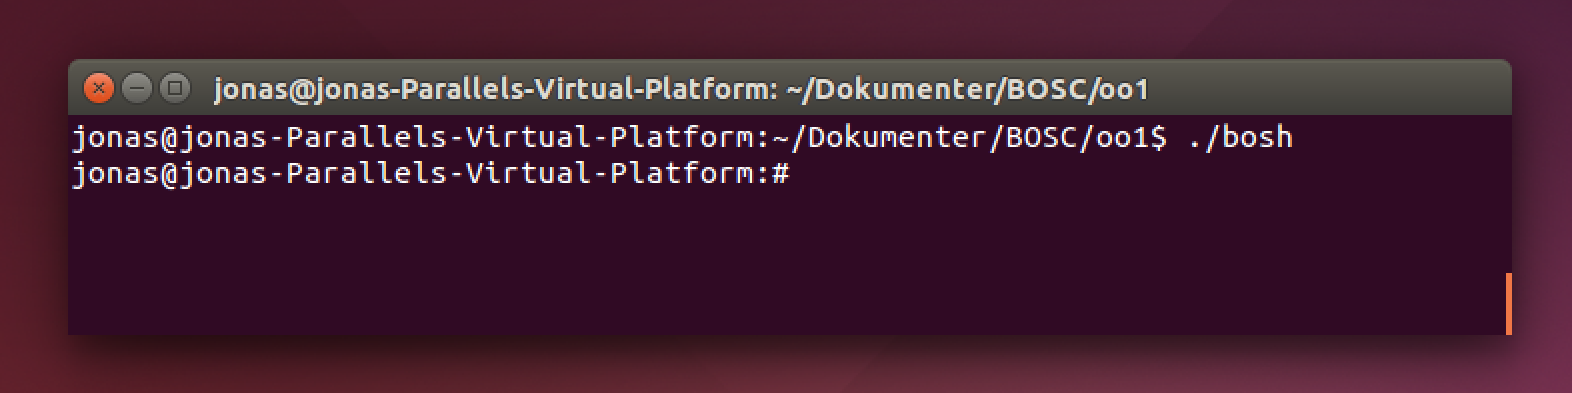
\includegraphics[width=0.95\textwidth]{opstart.png}}
\caption{bosh skriver brugernavn og værtsnavn til terminalen.}
\label{fig:opstart}
\end{figure}

\subsection{Simple eksekveringer - $K3$}
Vi bruger \texttt{execvp} funktionen til at køre kommandoer indtastet af brugern. \texttt{Execvp} leder efter den angivne kommando i \texttt{\$PATH} miljøet på maskinen. Ved at bruge denne kommando er vi i stand til at eksekvere simple kommandoer. 

\subsection{Ukendte funktioner - $K4$}
Hvis \texttt{execvp} ikke finder den kommando den får som parameter i \texttt{\$PATH} miljøet bliver kontrollen returneret til den process hvorfra \texttt{execvp} blev kaldt. Denne adfærd har vi udnyttet til fortæller brugeren hvis en given kommando ikke blev fundet. Ved at lade fejlmeddelelsen være det eneste kode, som er placeret efter kaldet til \texttt{execvp} vil dette kun bliver eksekveret hvis kommandoen ikke blev fundet. Efter at fejlmeddelelsen er skrevet til terminalen benytter vi \texttt{exit()} funktionen til at forhindre at barneprocessen forlader \texttt{executionshellcmd} funktionen og begynder at lytte efter nye brugerinput.

\subsection{Baggrundsprocesser - $K5$}
For at understøtte kravet om at kommandoer skulle kunne køres som baggrundsprocesser har vi brugt en simpel if sætning til at styre hvorvidt forælder processen skal vente eller ej. For at afgøre om forældre processen skal vente tjekker vi om $background$ feltet på shellcmd objektet er sat til sand(1). Hvis dette er tilfældet venter forældreprocessen på at barne processen returnere ellers fortsætter forælderprocessen og gør klar til at modtage en ny kommando. Dette gør det muligt at eksekvere flere kommandoer samtidig.  I figur~\ref{fig:background}, side~\pageref{fig:background}, ses et eksempel hvor flere kommandoer eksekveres som baggrundsprocesser samtidig.

\begin{figure}[H]
\center
\fbox{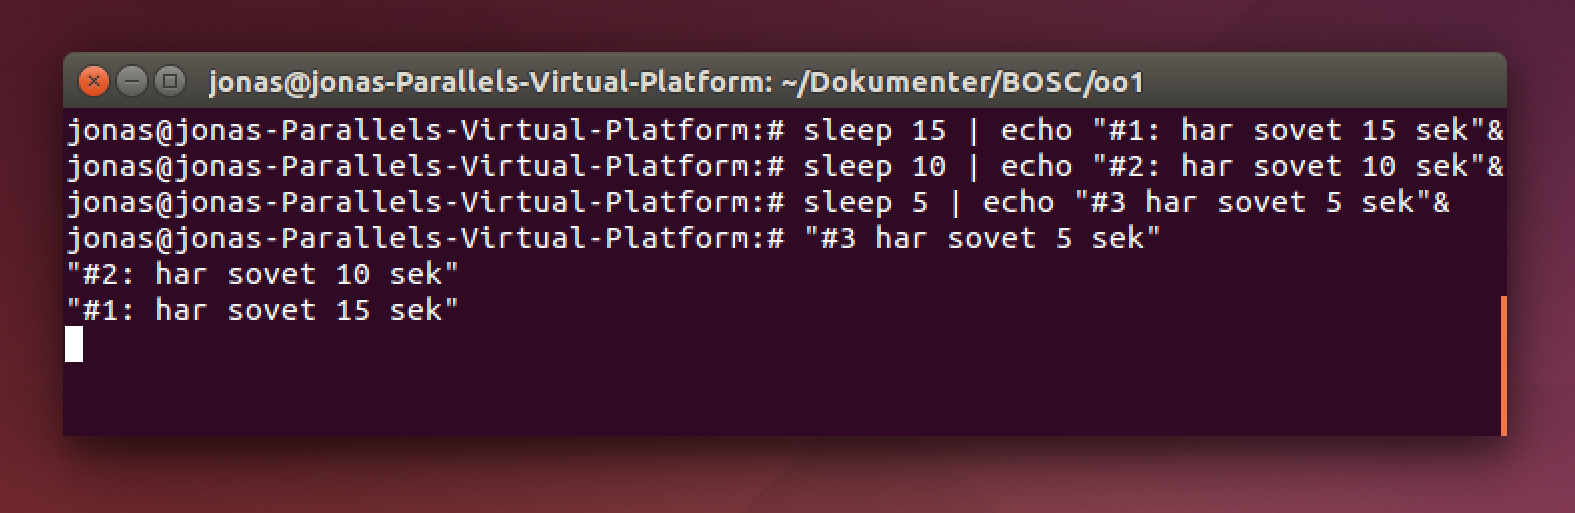
\includegraphics[width=0.95\textwidth]{background.png}}
\caption{bosh skriver brugernavn og værtsnavn til terminalen.}
\label{fig:background}
\end{figure}

\subsection{Standard I/O - $K6$}
Krav nr. 6 specificere at det skal være muligt at omdirigere kommandoens standard input og output således at det er muligt at læse input fra, samt at skriver output til filer. Til at opnå dette har vi gjort brug af \texttt{dup2} og \texttt{freopen}. \texttt{Dub2} gør det muligt at udskifte en standard I/O stream med en anden, mens \texttt{freopen} gør det muligt at genåbne stdin/stdout som en anden fil.\\
Når vores første barneproces bliver oprette tjekker vi først om brugeren har specificeret en input fil. Er dette tilfældet genåbner vi den specificerede fil som stdin. Her efter tjekker vi om der er angivet en output fil. Er dette også tilfældet åbner også denne fil og ændre processen stdout til filen, ved hjælp af \texttt{dub2}. Når dette er gjort fortsætter eksekveringen af bruger inputtet. 

\subsection{Kommandosekvenser - $K7$}
Som det fremgår af krav 7 skal det være muligt at sammenkæde kommandoer ved hjælp af $pipe$ operatoren "\textbar". Betydningen af denne operator er at resultatet af kommandoen på operatorens venstre side skal bruges input til kommandoen på operatorens højre side. Et eksempel på en sådan kommandosekvens kan ses i figur~\ref{fig:background} side~\pageref{fig:background}.\\

Vi har implementeret sammenkædningsfunktionaliteten ved hjælp af $pipe$ strukturen fra $unistd$ bibliotektet. Som nævnt i den overordnede beskrivelse af implementationen bliver kommandoerne parset i omvendt rækkefølge således at den kommando der ligger forrest i shellcmd objektet er den kommando som brugeren indtastede sidst. For at kæde kommandoerne sammen deler vi processen rekursivt så længe at der er flere kommandoer tilbage i shellcmd, på den måde ender vi med lige så mange barneprocesser som der er kommandoer i inputet. Hver gang en proces deles opretter vi en ‘pipe’, ændre standard inputet på forældre process til at være læse-enden af pipen, og ændre barneprocessens output til at være skrive-enden af pipen. Her efter venter forældreprocessen på at barneprocessen terminere mens barneprocessen arbejder videre med de resterende kommandoer. På den måde sikre vi os at kommandoerne eksekveres i den rigtige rækkefølge. 

\subsection{Quit on exit - $K8$}
For dette krav har vi valgt en simpel og direkte fremgangsmåde. Når metoden \texttt{initialExecution} køres, checkes om indholdet af den sidst indtastede kommando matcher strengene $'exit'$ og $'quit'$. Gør den det, returnerer metoden med value $0$, hvilket afbryder \texttt{while} løkken og programmet standser ved at returnere \texttt{EXIT\_SUCCESS}.

Se afsnit~\ref{sec:fm} 'Fejl og mangler' side~\pageref{sec:fm} for yderligere oplysninger.

\subsection{Interrupt - $K9$}
For at undgå at bosh terminere når brugeren benytter tastekombinationen "CTRL + C", men at bosh i stedet terminere alle sine barneprocesser har vi tilføjet to signal handlers. Den første handler, parent\_int, linje 27 - 29, bliver brugt at forældre processen når den modtager et signal af typen \texttt{SIGINT}. Handleren skriver en besked til skærmen om at børne processer bliver termineret, hvor efter den returnere kontrollen til brugeren. 
Den anden handler, child\_int, linje 23 - 25, bliver benyttet af alle børeneprocesser. Handleren lukker den aktuelle process og på den måde bliver alle processer med undtagelse af forældreprocessen lukket. For at sikre at forældreprocessen ikke anvender den forkerte handler bliver child\_int først sat efter at forældreprocessen bliver delt.\\

\section{Fejl og mangler}
\label{sec:fm}
På grund af den måde exit-funktionaliteten er implementeret ($K8$), er der begrænsninger på hvilke situationer exit kommandoen fungerer. Vi foretager et check i \texttt{initialExecution} metoden, hvilket betyder at vi reelt kun undersøger den første kommando i \_shellcmd structen, dvs. den sidst indtastede kommando i en given kommandolinie. Samtidigt betyder det, at programmet terminerer uden at eksekvere nogen anden kommando.\\

Det kan argumenteres at dette ikke er den optimale løsning, i det der kunne være situationer hvor en ønsker at sætte en serie af lange operationer til at køre, for til sidst at lukke bosh ned. Vores løsning understøtter på nuværende tidspunkt ikke denne funktionalitet, selvom det formelle krav om at konstruere en exit-funktion til at lukke programmet er opfyldt.

\end{document}